\documentclass[border=4pt]{standalone}
\usepackage{amsmath,amssymb,amsfonts}
\usepackage{xcolor,colortbl,array,booktabs,multirow}
\usepackage{tikz}
\usepackage{pgfplots}
\pgfplotsset{compat=1.16}
\usetikzlibrary{arrows, automata, backgrounds, calendar, chains, decorations,
    matrix, mindmap, patterns, petri, positioning, shadows, shapes.geometric,
    trees, shapes, decorations.pathreplacing, calc, tikzmark, arrows.meta,
    intersections, fit, graphs, quotes, angles, decorations.markings}
\newcommand{\st}{\text{ s.t. }}
\newcommand{\x}{\mathbf{x}}
\renewcommand{\b}{\mathbf{b}}
\renewcommand{\c}{\mathbf{c}}
\newcommand{\A}{\mathbf{A}}
\newcommand{\y}{\mathbf{y}}
\newcommand{\z}{\mathbf{z}}
\newcommand{\R}{\mathbb{R}}
\newcommand{\RR}{\mathbb{R}}
\newcommand{\Z}{\mathbb{Z}}
\newcommand{\ZZ}{\mathbb{Z}}
\newcommand{\npcomplete}{NP-complete}
\providecommand{\true}{\text{TRUE}}
\providecommand{\false}{\text{FALSE}}
\tikzset{vertex/.style={circle,fill=black!25,minimum size=20pt,inner sep=0pt},
    edge/.style={draw,thick,-},weight/.style={font=\small},
    selected vertex/.style={vertex, fill=red!24},
    selected edge/.style={draw,line width=2pt,-,red!50},
    ignored edge/.style={draw,line width=2pt,-,black!20}}
\newcommand{\vect}{\vec}
\providecommand{\ds}{\displaystyle}
\providecommand{\longvect}{\overrightarrow}
\usepackage[normalem]{ulem}
\definecolor{ocre}{RGB}{243,102,25}
\providecommand{\leftB}{\left[}
\providecommand{\rightB}{\right]}
\tikzset{directed/.style={postaction={decorate,decoration={markings,mark=at position .65 with {\arrow{>}}}}},
    directed1/.style={postaction={decorate,decoration={markings,mark=at position .65 with {\arrow{>}}}}}}
\begin{document}
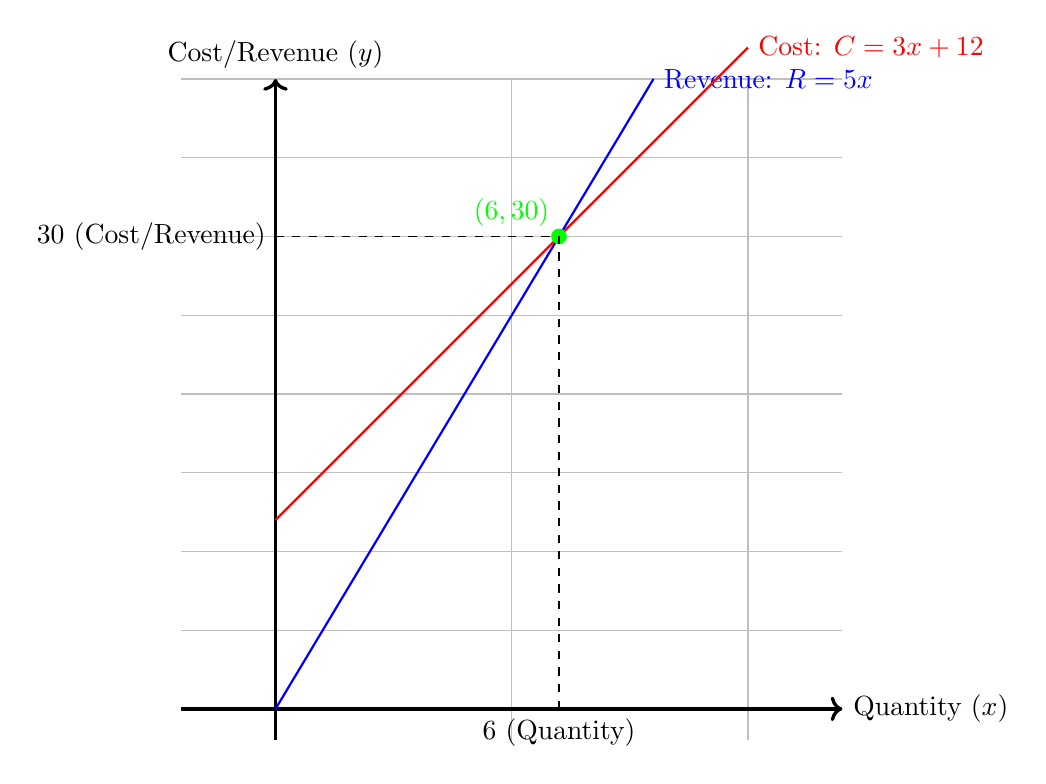
\begin{tikzpicture}[xscale=0.6, yscale=0.2]

    % Grid and axes
    \draw[gray!50, thin, step=5] (-2,-2) grid (12,40);
    \draw[very thick,->] (-2,0) -- (12,0) node[right] {Quantity ($x$)};
    \draw[very thick,->] (0,-2) -- (0,40) node[above] {Cost/Revenue ($y$)};

    % Revenue line: R = 5x
    \draw[blue, thick] (0,0) -- (8,40) node[anchor=west] {Revenue: $R=5x$};

    % Cost line: C = 3x + 12
    \draw[red, thick] (0,12) -- (10,42) node[anchor=west] {Cost: $C=3x+12$};

    % Break-even point
    \node[green] at (6,30) [circle,fill,inner sep=2pt]{};
    \node[green,anchor=south east] at (6,30) {$(6,30)$};

    % Vertical and horizontal dashed lines to axes
    \draw[dashed] (6,0) -- (6,30);
    \draw[dashed] (0,30) -- (6,30);

    % Labels for break-even
    \node[anchor=north] at (6,0) {6 (Quantity)};
    \node[anchor=east] at (0,30) {30 (Cost/Revenue)};
\end{tikzpicture}
\end{document}
